% file: transitive.tex

\documentclass{standalone}

\usepackage{tikz}
\usetikzlibrary{arrows.meta, positioning}

\begin{document}
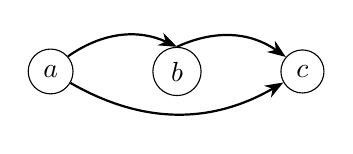
\begin{tikzpicture}[every node/.style = {draw, circle, minimum size = 10pt},
  relation/.style = {>=Stealth, ->, thick}]
  \node (a) [] {$a$};
  \node (b) [right = 1.0cm of a] {$b$};
  \node (c) [right = 1.0cm of b] {$c$};

  \draw [relation, bend left] (a) to (b.north);
  \draw [relation, bend left] (b.north) to (c);
  \draw [relation, bend right] (a) to (c);
\end{tikzpicture}
\end{document}

